\chapter{Specifikace požadavků}
\label{ch:specifikace}

\section{Funkce aplikace}

Aplikace má pět částí:
\parskip=0em
\begin{itemize}
	\item Medikační karta
	\item Denní bilance tekutin
	\item Hodinová bilance tekutin
	\item Invazivní přístupy
	\item Fyziologie
\end{itemize}
\parskip=1em

Medikační karta nahrazuje tištěnou medikační kartu. Její vzhled odpovídá tištěné formě (tabulka se seznamem léků a jednotlivými hodinami). Podání ordinovaného léku se bude moci provést DoubleClickem, nebo se jednoduchým kliknutím zobrazí dialog, ve kterém může uživatel editovat jednotlivé ordinace daného léku.

Denní bilance tekutin odpovídá bilanci tekutin ve WinMedicalcu. Umožňuje zadávat množství příjmu a výdeje tekutin (celkovou hodnotu nebo nově naměřenou hodnotu).

Hodinová bilance tekutin je podobná denní bilanci tekutin. Ukazuje příjem a výdej tekutin v danou hodinu. Dále umožňuje zobrazit příjem a výdej tekutin ve všech hodinách.

Záložka invazivních přístupů odpovídá invazivním přístupům ve WinMedicalcu. Zobrazuje zavedené invazivní přístupy a jejich popis. Umožňuje přístupy editovat, označit požadavkem na výměnu, přidat a smazat.

Záložka fyziologie zobrazuje záznamy životních funkcí pacienta. Záznamy lze přidat, editovat, nebo smazat.


\section{Kontext systému}

Aplikace je kompatibilní s informačím systémem FN Plzeň. Doplňuje aplikaci WinMedicalc, systémová integrita mezi oběmi aplikacemi není. Data jsou uložena v Oracle databázi nemocnice.

S vyvíjenou aplikací budou pracovat výhradně zdravotní sestry. Použití aplikace MediTab a WinMedicalc znázorňuje kontextový diagram na obrázku \ref{fig:kontext}.

\begin{figure}[H]
	\centering
	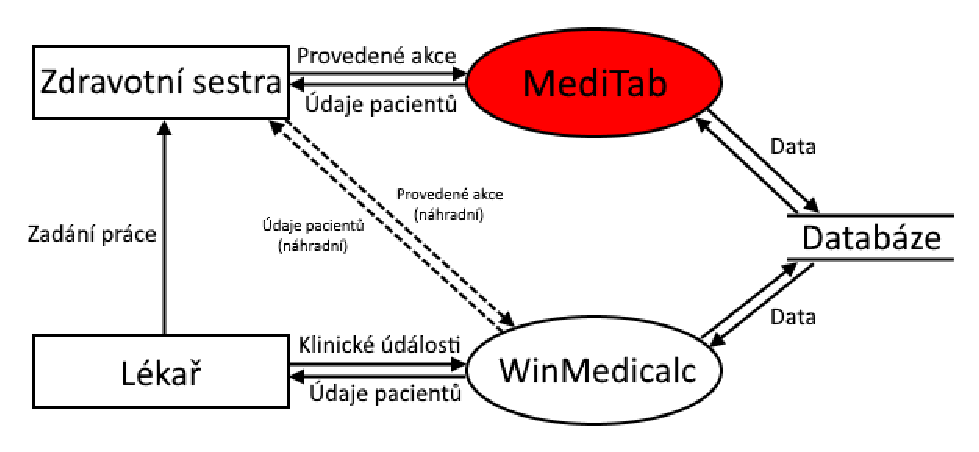
\includegraphics[width=0.8\textwidth]{img/kontext.eps}
	\caption{Kontextový diagram}
  \label{fig:kontext}
\end{figure}


\section{Technické parametry}

Aplikace běží na systému Microsoft Windows 8.1 64bit. Je vyvíjená na platformě Microsoft .NET Framework 4.5 v jazyce C\# \cite{msdn}.

Aplikace je kompatibilní s informačním systémem FN Plzeň a bude doplňovat program WinMedicalc. Systémová integrita mezi oběmi aplikacemi není, pouze jsou využity některé funkční prvky WinMedicalcu.

\subsection{Tablet}

SIS FN Plzeň vybralo HP ElitePad 1000G2 Healthcare Tablet, který je schválený pro použití v nemocničním prostředí. Tento tablet má antibakteriální povrchovou úpravu a odolnější konstrukci.

\noindent
Specifikace:

\noindent
\begin{tabular}{l l}
	Operační systém: & Microsoft Windows 8.1 64bit\\
	Procesor: & Intel Atom Z3795 (1.6 GHz, 2 MB cache, 4 jádra)\\
	Operační paměť: & 4 GB LPDDR3 SDRAM (1067 MHz)\\
	Interní paměť: & 128 GB eMMC\\
	Grafická karta: & Intel HD Graphics\\
	Displej: & 10.1" 1920 x 1200 (WUXGA)\\
	Výstupy: & 1 x USB 3.0, 1 x HDMI
\end{tabular}


\section{Databáze}

Přístup do databáze FN Plzeň je pouze ze zařízení, které jsou připojeny k~doméně FN Plzeň. Proto byla část databáze potřebná pro vývoj aplikace zkopírována do nového tablespace v Oracle databázi na ZČU. Tabulky, ke kterým aplikace MediTab přistupuje jsou v ERA modelu na obrázku \ref{fig:era}. Kopie databáze je naplněna fiktivními testovacími daty, které odpovídají realným datům.

\begin{figure}[H]
	\centering
	\includegraphics[width=1\textwidth]{img/ERA.eps}
	\caption{ERA model části databáze k vývoji aplikace}
  \label{fig:era}
\end{figure}
